% =====================================================================
%  Model-Based Fault Detection and Isolation for Robot Joint Actuators
%  Draft v0.2  (simulation study complete; hardware section is a placeholder)
%  Target: IEEE/ASME AIM (6 pages, IEEEtran conference). Also fits IECON,
%  SAFEPROCESS (reformat to IFAC), or RA-L (expand the hardware section).
%
%  All simulation numbers come from sim/run_experiments.py
%  (results in sim/results/results.json). Rerun it after changing
%  parameters and update the numbers below.
% =====================================================================
\documentclass[conference]{IEEEtran}
\IEEEoverridecommandlockouts

\usepackage{amsmath,amssymb,amsfonts}
\usepackage{graphicx}
\usepackage{booktabs}
\usepackage{siunitx}
\usepackage{xcolor}
\usepackage{tikz}
\usetikzlibrary{arrows.meta,positioning,calc,fit}
\usepackage{cite}
\usepackage[hidelinks]{hyperref}
\usepackage[capitalise,nameinlink]{cleveref}

% ---------- drafting helpers (delete before submission) ----------
\newcommand{\TBD}[1]{\textcolor{red}{[TBD: #1]}}
\newcommand{\NOTE}[1]{\textcolor{blue}{[Note: #1]}}
\newcommand{\FIGPH}[2]{%
  \fbox{\parbox[c][#1][c]{0.94\linewidth}{\centering\small\ttfamily #2}}}

\begin{document}

\title{Isolating Sensor Faults from Mechanical Events in Robot Joint Actuators
Using Back-EMF and Momentum Residuals\\
\thanks{\TBD{funding / acknowledgment}}}

\author{\IEEEauthorblockN{Lakshanand Sugumar}
\IEEEauthorblockA{\textit{\TBD{School / Department}} \\
\textit{Arizona State University}\\
Tempe, AZ, USA \\
\TBD{email}}
\and
\IEEEauthorblockN{\TBD{Faculty co-advisor}}
\IEEEauthorblockA{\textit{\TBD{School / Department}} \\
\textit{Arizona State University}\\
Tempe, AZ, USA \\
\TBD{email}}}

\maketitle

% =====================================================================
\begin{abstract}
A joint actuator that stops on every anomaly is safe but unusable, and one
that ignores anomalies is dangerous; the right reaction depends on whether the
fault is in the sensor or in the mechanics. We present a model-based fault
detection and isolation (FDI) scheme for permanent-magnet synchronous motor
(PMSM) joint actuators that separates the two classes using only signals the
field-oriented control (FOC) loop already computes. A back-EMF voltage residual,
built from the commanded $dq$ voltages, measured currents, and encoder speed,
responds to encoder faults but is structurally insensitive to load torque. A
generalized-momentum observer responds to external torque but is trusted only
while the voltage residual certifies the encoder. Together with a short
angle-free voltage-pulse test, the residuals isolate encoder faults, phase open
circuits, collisions, and load changes, and select a class-specific reaction.
In a simulation study with model errors of up to \SI{30}{\percent}, 300
Monte Carlo fault trials, and one hour of normal motion, the scheme isolated
299 of 300 faults with no false alarms. Encoder faults raised an alarm within
\SI{0.51}{\milli\second} and were isolated in a median of
\SI{3.5}{\milli\second}; collisions were detected in a median of
\SI{2.3}{\milli\second} against \SI{7.0}{\milli\second} for a following-error
check, which also raised false alarms in \SI{22}{\percent} of normal runs.
\TBD{One sentence on hardware results.}
\end{abstract}

\begin{IEEEkeywords}
fault detection and isolation, PMSM, encoder fault, collision detection,
momentum observer, robot joint actuator, humanoid robots
\end{IEEEkeywords}

% =====================================================================
\section{Introduction}
\label{sec:intro}

Legged and humanoid robots are built from compact, highly geared or
quasi-direct-drive joint actuators that run FOC at tens of kilohertz
\cite{wensing2017proprioceptive,katz2019minicheetah}. Each actuator is a single
point of failure: if the knee of a humanoid stops producing torque, the robot
falls. At the same time, these actuators interact physically with people and
the environment, so contacts must be detected fast enough to bound the contact
force \cite{haddadin2017collisions}.

Most drives handle both problems with a small set of generic checks: hardware
encoder error flags, over-current trips, and a following-error limit on
$|q_\mathrm{ref}-\hat q|$. These checks have two weaknesses. First, they are
slow or blind for an important class of faults: an encoder that
\emph{freezes} or \emph{slips} (for example, a shifted magnet, a stuck SPI
read, or a corrupted but CRC-valid frame) raises no flag at all. Second, they
do not \emph{isolate}: a large following error can be caused by a collision,
by a heavy payload, or by a wrong encoder angle that misaligns the current
vector. These events call for opposite reactions. A collision calls for
compliance, a payload change calls for compensating the load, and an encoder
fault calls for leaving angle-dependent control, because any reaction that
trusts the encoder will make things worse.

This paper asks whether a joint actuator can tell a sensor fault from a
mechanical event using only signals the FOC loop already has, without
additional sensors. Our answer is a pair of residuals with complementary
sensitivity:
\begin{itemize}
  \item a \emph{back-EMF voltage residual} $r_v$ that compares the commanded
  $dq$ voltages with those predicted by the electrical model at the
  encoder-reported speed and angle. Load torque changes the current, but the
  model accounts for the current, so $r_v$ is insensitive to load; an encoder
  error changes the predicted back-EMF, so $r_v$ is sensitive to encoder faults.
  \item a \emph{generalized-momentum observer} $r_m$
  \cite{deluca2003actuator,deluca2006collision} that estimates the external
  joint torque. It responds to collisions and payload changes. It also reacts
  to encoder faults, because it uses the encoder speed, so its output is
  interpreted only while $r_v$ is quiet.
\end{itemize}

\textbf{Contributions.}
(i) A structured residual design for PMSM joint actuators that decouples
encoder faults from external torque using only FOC signals
(\cref{sec:method}); (ii) a decision logic, including an angle-free
voltage-pulse test, that isolates four fault classes and maps each to a
reaction (\cref{sec:isolation}); (iii) a simulation study with model error,
Monte Carlo fault injection, long normal runs, and ROC analysis against a
following-error baseline (\cref{sec:sim}); and (iv) a hardware validation on
\TBD{actuator name} with injected encoder faults, phase open circuits, and
collisions at several speeds (\cref{sec:hw}).

% =====================================================================
\section{Related Work}
\label{sec:related}

\textbf{Model-based FDI.} Residual generation with structured sensitivity is a
classical tool for isolation
\cite{gertler1998fault,chen1999robust,isermann2006fault,blanke2016diagnosis}.
Our contribution is not a new observer class but a residual pair whose
structural decoupling follows from the physics of the PMSM and joint, chosen
so that it fits in the existing FOC interrupt.

\textbf{Collision detection in robots.} The generalized-momentum observer of
De~Luca \emph{et al.} \cite{deluca2003actuator,deluca2006collision} is the
standard sensorless approach for manipulators and is surveyed in
\cite{haddadin2017collisions}. These works assume healthy joint position
sensing; we add a residual that certifies this assumption at run time.

\textbf{Position sensor faults in PMSM drives.} Sensor fault detection and
tolerant control for electric drives has been studied mostly for traction and
industrial drives \cite{akrad2011fault,bourogaoui2016speed}, often by comparing
the encoder with a sensorless estimate based on back-EMF
\cite{chen2003extended,matsui1996sensorless}. Open-phase faults and
fault-tolerant topologies are reviewed in \cite{welchko2004fault}.
\TBD{Add 3--5 recent (2022--2026) papers on actuator-level FDI and
fault-tolerant control for legged or humanoid robots from IEEE Xplore, and
position the gap: joint-level isolation of sensor versus mechanical faults
using only FOC signals.}

% =====================================================================
\section{System Model}
\label{sec:model}

\subsection{Electrical model}
In the rotor reference frame, a surface PMSM obeys
\begin{align}
  v_d &= R\,i_d + L_d\,\dot i_d - \omega_e L_q\, i_q, \label{eq:vd}\\
  v_q &= R\,i_q + L_q\,\dot i_q + \omega_e\,(L_d\, i_d + \lambda_m), \label{eq:vq}
\end{align}
where $R$ is the phase resistance, $L_{d,q}$ the inductances, $\lambda_m$ the
permanent-magnet flux linkage, and $\omega_e = p\,\dot\theta_m$ the electrical
speed for $p$ pole pairs. The FOC loop computes the $dq$ quantities with the
\emph{measured} electrical angle $\hat\theta_e = p\,\hat\theta_m$. We write
$\delta = \theta_e - \hat\theta_e$ for the angle error and
$\hat\omega_e$ for the speed derived from the encoder.

\subsection{Mechanical model}
With gear ratio $N$, torque constant $k_t = \tfrac{3}{2}p\lambda_m$, and
reflected inertia $J$, the joint obeys
\begin{equation}
  J\,\ddot q = \tau_m - \tau_f(\dot q) - \tau_g(q) + \tau_\mathrm{ext},
  \qquad \tau_m = N k_t\, i_q, \label{eq:mech}
\end{equation}
where $\tau_f$ is friction, $\tau_g$ a known gravity or spring term (zero for
a horizontal joint), and $\tau_\mathrm{ext}$ the unknown external torque from
contact or payload.

\subsection{Fault classes}
We consider four classes, summarized in \cref{tab:faults}:
\textsc{Enc} (encoder freeze, offset/slip, or disconnect),
\textsc{Phase} (open circuit of one motor phase),
\textsc{Coll} (transient external torque from contact), and
\textsc{Load} (persistent change in external torque, e.g.\ a payload).

% =====================================================================
\section{Residual Design}
\label{sec:method}

\subsection{Back-EMF voltage residual}
Let $v^*_{dq}$ be the voltages commanded by the current controllers (available
in the FOC loop before modulation). The model-predicted voltage at the
encoder speed is
\begin{equation}
  \hat v_{dq} = R\,i_{dq} + L\,\dot i_{dq}
   + \hat\omega_e \begin{bmatrix} -L_q i_q \\ L_d i_d + \lambda_m \end{bmatrix},
\end{equation}
and the residual is $r_v = v^*_{dq} - \hat v_{dq}$. Neglecting inverter
nonlinearity and parameter error for the moment, and expressing the true
back-EMF in the frame defined by $\hat\theta_e$, gives
\begin{equation}
  r_v \approx \lambda_m
  \begin{bmatrix} -\omega_e \sin\delta \\ \omega_e\cos\delta - \hat\omega_e \end{bmatrix}.
  \label{eq:rv}
\end{equation}
Two properties follow directly from \cref{eq:rv}:
\begin{enumerate}
  \item \emph{Load insensitivity.} $\tau_\mathrm{ext}$ enters only through
  $i_{dq}$, which is measured and compensated in $\hat v_{dq}$. Hence
  $r_v \approx 0$ for any load when $\delta = 0$ and
  $\hat\omega_e = \omega_e$.
  \item \emph{Encoder sensitivity.} An angle offset ($\delta\ne0$) gives
  $\|r_v\|\approx 2\lambda_m|\omega_e\sin(\delta/2)|$, and a frozen encoder
  ($\hat\omega_e \to 0$, $\delta$ growing) gives
  $\|r_v\|\approx\lambda_m|\omega_e|$.
\end{enumerate}
To avoid differentiating noisy currents, $r_v$ is computed after a first-order
low-pass filter $F(s)=a/(s+a)$ applied to both $v^*$ and the model, with the
$L\,\dot i$ term computed as $L\,a\,(i - F i)$. Unmodeled terms, mainly
dead-time voltage error, thermal drift of $R$, and error in $\lambda_m$, are
bounded by a threshold that follows their structure:
\begin{equation}
  \|r_v\| > \tau_v = c_0 + c_1|\hat\omega_e| + c_2\|i_{dq}\|. \label{eq:thr_v}
\end{equation}
We set $c_1 = 1.5\,\Delta\lambda_m$ and $c_2 = 1.5\,\Delta R$ from the
assumed parameter-error bounds, and $c_0$ to 1.25 times the largest remaining
residual over a calibration set of normal motion (\cref{sec:sim}).
Because the fault signature scales with $|\omega_e|$, a frozen encoder is
detectable only above $|\omega_e| > c_0/(\lambda_m - c_1)$. A frozen reading at
standstill is correct until the joint moves, so this limit mostly delays
detection until motion starts (\cref{sec:sim}).

\subsection{Generalized-momentum observer}
Following \cite{deluca2003actuator}, define the momentum $\rho = J\dot q$ and
the residual
\begin{equation}
  r_m(t) = K\!\left[\rho(t) - \!\int_0^t\!\big(\tau_m - \hat\tau_f(\dot q)
   - \tau_g(q) + r_m\big)\,ds - \rho(0)\right], \label{eq:mo}
\end{equation}
with gain $K>0$. Substituting \cref{eq:mech} gives
$\dot r_m = K(\tau_\mathrm{ext} - r_m)$, so $r_m$ is a first-order
filtered estimate of $\tau_\mathrm{ext}$ (plus friction and inertia model
error) with bandwidth $K$, and needs no acceleration measurement. An alarm is
raised when $|r_m| > \tau_m^\mathrm{thr}$.

The observer uses $\dot q$ from the encoder, so an encoder fault corrupts
$r_m$: a freeze makes $\rho$ drop to zero and $r_m$ shows a spurious torque.
In simulation $r_m$ often alarms \emph{before} $r_v$ on an encoder freeze
(\cref{fig:sim_enc}). This is why $r_m$ alone cannot isolate, and why the
logic below waits briefly for $r_v$ before acting on a mechanical label.

\subsection{Discrete implementation}
Both residuals run at the current-loop rate $f_s=\SI{20}{\kilo\hertz}$ and
need roughly 30 multiply-accumulates per cycle on top of FOC (our estimate). Each alarm requires
$n_d = 5$ consecutive samples (\SI{0.25}{\milli\second}) over threshold.
\TBD{Report the measured CPU time added to the FOC interrupt on the target
MCU.}

% =====================================================================
\section{Fault Isolation and Reaction}
\label{sec:isolation}

\Cref{tab:faults} is the structure (incidence) matrix of the residual set,
extended with the reaction for each class.

\begin{table}[t]
\centering
\caption{Fault signatures and reactions. \checkmark: residual fires;
0: residual stays below threshold; $\ast$: may fire but is not trusted.}
\label{tab:faults}
\setlength{\tabcolsep}{3pt}
\begin{tabular}{@{}lcccl@{}}
\toprule
Class & $r_v$ & $r_m$ & pulse test & Reaction \\
\midrule
\textsc{Enc}   & \checkmark & $\ast$ & balanced & ASC \\
\textsc{Phase} & \checkmark & $\ast$ & one phase dead & ASC \\
\textsc{Coll}  & 0 & transient & -- & zero torque \\
\textsc{Load}  & 0 & persistent & -- & resume + feedforward \\
\bottomrule
\end{tabular}
\end{table}

The logic is evaluated every cycle:
\begin{enumerate}
  \item \emph{$r_v$ alarm.} The encoder or the electrical path is suspect, so
  $r_m$ is disregarded and the inverter enters active short circuit (ASC), a
  standard safe state for PMSM drives that needs no rotor angle. After
  \SI{2}{\milli\second} of settling, three \SI{0.1}{\milli\second},
  \SI{2}{\volt} voltage pulses are applied along the $a$, $b$, and $c$ phase
  axes in the stationary frame, again without the rotor angle. If one phase's
  current response is below \SI{30}{\percent} of the median response, the
  class is \textsc{Phase}; otherwise it is \textsc{Enc}.
  \item \emph{$r_m$ alarm, $r_v$ quiet.} The event is treated as a possible
  collision at once: the torque command is set to zero (compliant). If $r_v$
  alarms within the next \SI{40}{\milli\second}, step 1 takes over. After
  $T_\mathrm{coll}=\SI{40}{\milli\second}$ the class is \textsc{Load} if
  $|r_m|$ is still above threshold, and position control resumes with $-r_m$
  as torque feedforward; otherwise the class is \textsc{Coll} and the joint
  stays compliant.
  \item Otherwise the actuator is healthy.
\end{enumerate}
Reacting on the first $r_m$ alarm keeps the collision reaction latency equal to
the detection latency, at the cost of briefly releasing a payload before it is
recognized as \textsc{Load}.

\begin{figure}[t]
\centering
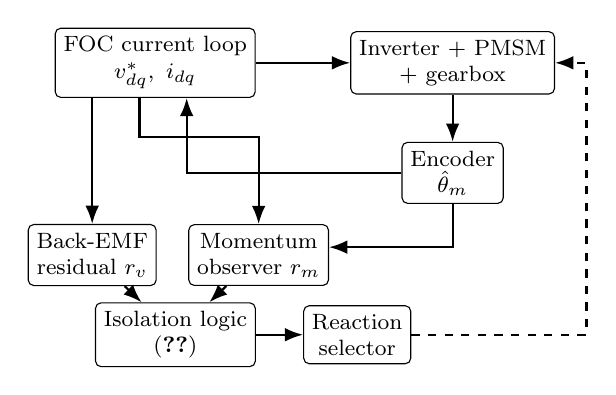
\begin{tikzpicture}[
  font=\footnotesize, >=Latex,
  blk/.style={draw, rounded corners=2pt, minimum height=6mm, align=center, inner sep=3pt},
  sig/.style={->, thick}]
  \node[blk] (foc) {FOC current loop\\$v^*_{dq},\ i_{dq}$};
  \node[blk, right=12mm of foc] (pmsm) {Inverter + PMSM\\+ gearbox};
  \node[blk, below=6mm of pmsm] (enc) {Encoder\\$\hat\theta_m$};
  \node[blk, below=16mm of foc, xshift=-8mm] (rv) {Back-EMF\\residual $r_v$};
  \node[blk, right=4mm of rv] (rm) {Momentum\\observer $r_m$};
  \node[blk, below=6mm of $(rv)!0.5!(rm)$] (iso) {Isolation logic\\(\cref{tab:faults})};
  \node[blk, right=6mm of iso] (react) {Reaction\\selector};
  \draw[sig] (foc) -- (pmsm);
  \draw[sig] (pmsm) -- (enc);
  \draw[sig] (enc.west) -| ($(foc.south)+(4mm,0)$);
  \draw[sig] ($(foc.south)-(8mm,0)$) -- ++(0,-3mm) -| (rv.north);
  \draw[sig] ($(foc.south)-(2mm,0)$) -- ++(0,-5mm) -| (rm.north);
  \draw[sig] (enc.south) |- ($(rm.east)+(0,1mm)$);
  \draw[sig] (rv) -- (iso);
  \draw[sig] (rm) -- (iso);
  \draw[sig] (iso) -- (react);
  \draw[sig, dashed] (react.east) -| ($(pmsm.east)+(4mm,0)$) -- (pmsm.east);
\end{tikzpicture}
\caption{FDI architecture. Both residuals use only signals already present in
the FOC loop; no sensors are added.}
\label{fig:arch}
\end{figure}

% =====================================================================
\section{Simulation Study}
\label{sec:sim}

\subsection{Setup}
The simulation models a small quasi-direct-drive actuator
(\cref{tab:params}): a surface PMSM in the stationary frame integrated at
\SI{100}{\kilo\hertz}; a three-phase inverter with \SI{0.1}{\volt}
dead-time voltage error; a 14-bit motor-side encoder; current-sensor noise
of \SI{30}{\milli\ampere} rms; viscous and Coulomb friction; FOC at
\SI{20}{\kilo\hertz} with \SI{1.5}{\kilo\hertz} current loops; and a
\SI{10}{\hertz} PD position loop with model feedforward, all driven by the
measured encoder angle. The speed estimate is a filtered encoder difference
(\SI{300}{\hertz}). Contacts are a spring-damper obstacle
(\SI{100}{\newton\metre\per\radian}). The controller and the residuals use a
model whose parameters differ from the plant by uniform random errors of up to
$\pm\SI{20}{\percent}$ on $R$, $\pm\SI{5}{\percent}$ on $\lambda_m$,
$\pm\SI{10}{\percent}$ on $J$ and $L$, and $\pm\SI{30}{\percent}$ on both
friction coefficients, drawn anew for every run. The parameters are
representative values, not identified from our testbed.
\NOTE{Replace with identified testbed parameters and rerun.}

\textbf{Thresholds} were calibrated once on 3 minutes of normal motion (sine,
chirp to \SI{4.5}{\hertz}, and random minimum-jerk moves up to
\SI{6}{\radian\per\second}) and then frozen: $c_0=\SI{0.23}{\volt}$,
$c_1=\SI{4.5e-4}{\volt\second\per\radian}$, $c_2=\SI{0.09}{\volt\per\ampere}$,
$\tau_m^\mathrm{thr}=\SI{0.093}{\newton\metre}$. The baseline following-error
check was calibrated the same way (1.25 times the largest value seen),
giving \SI{6.2}{\milli\radian}.

\begin{table}[t]
\centering
\caption{Simulated actuator parameters (representative, not identified)}
\label{tab:params}
\begin{tabular}{@{}lll@{}}
\toprule
Parameter & Symbol & Value \\
\midrule
Pole pairs & $p$ & 14 \\
Phase resistance & $R$ & \SI{0.30}{\ohm} \\
$d$/$q$ inductance & $L_d=L_q$ & \SI{100}{\micro\henry} \\
Flux linkage & $\lambda_m$ & \SI{6.0}{\milli\weber} \\
Gear ratio & $N$ & 6 \\
Joint-side inertia & $J$ & \SI{2.0e-3}{\kilo\gram\metre\squared} \\
Viscous / Coulomb friction & $b$, $\tau_c$ & \SI{0.01}{\newton\metre\second\per\radian}, \SI{0.05}{\newton\metre} \\
Bus voltage / current limit & -- & \SI{24}{\volt}, \SI{8}{\ampere} \\
Current-loop rate & $f_s$ & \SI{20}{\kilo\hertz} \\
Encoder resolution & -- & 14 bit (motor side) \\
Observer gain & $K$ & \SI{200}{\per\second} \\
Residual filter & $a$ & $2\pi\cdot\SI{500}{\radian\per\second}$ \\
\bottomrule
\end{tabular}
\end{table}

\subsection{Silent encoder freeze}
At $t=0$ the encoder output is held at its last value with no error flag while
the joint cruises at \SI{1}{\radian\per\second} (\cref{fig:sim_enc}). The
angle error $\delta$ grows with the true motion and $r_v$ crosses its threshold
after \SI{0.60}{\milli\second}. The momentum residual alarms even earlier, at
\SI{0.30}{\milli\second}, because the speed estimate collapses; acting on it
alone would mislabel the fault as a collision. The following-error check
alarms only after \SI{6.4}{\milli\second}, and it cannot say whether the
sensor or the mechanics failed.

\begin{figure}[t]
\centering
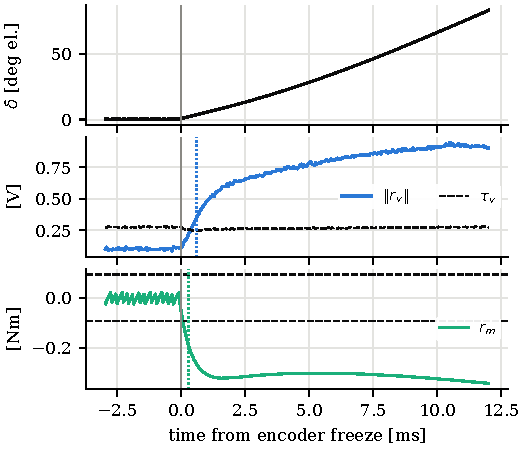
\includegraphics[width=\linewidth]{figures/sim_encoder_freeze.pdf}
\caption{Simulated silent encoder freeze at \SI{1}{\radian\per\second}.
Top: electrical angle error. Middle: back-EMF residual and its threshold.
Bottom: momentum residual and threshold. Dotted lines mark alarms.}
\label{fig:sim_enc}
\end{figure}

\subsection{Collision}
\Cref{fig:sim_coll} shows an impact at \SI{2}{\radian\per\second}. The
momentum observer detects the contact \SI{2.8}{\milli\second} after impact,
against \SI{7.9}{\milli\second} for the following-error check. With the
proposed reaction the peak contact torque is \SI{0.83}{\newton\metre}
against \SI{0.92}{\newton\metre} with the baseline; without any reaction the
position controller keeps pushing and the contact torque rises to the current
limit (\SI{6.1}{\newton\metre}) within \SI{0.4}{\second}. Throughout the
collision $\|r_v\|$ stays well below $\tau_v$, confirming the load
insensitivity predicted by \cref{eq:rv}.

\begin{figure}[t]
\centering
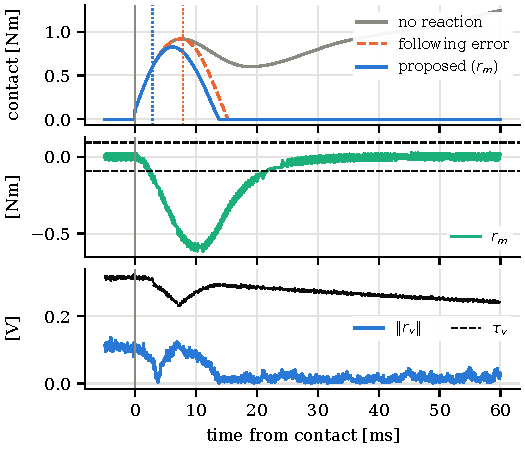
\includegraphics[width=\linewidth]{figures/sim_collision.pdf}
\caption{Simulated collision at \SI{2}{\radian\per\second}. Top: contact torque
with no reaction, the following-error check, and the proposed observer.
Middle: momentum residual. Bottom: back-EMF residual, which stays below its
threshold.}
\label{fig:sim_coll}
\end{figure}

\subsection{Effect of speed}
\Cref{fig:sim_sweep} sweeps the joint speed. Encoder-freeze detection by $r_v$
takes \SI{2.95}{\milli\second} at \SI{0.25}{\radian\per\second} and
\SI{0.40}{\milli\second} at \SI{4}{\radian\per\second}, against
\SIrange{25.7}{1.7}{\milli\second} for the following-error check. The
analytic limit $|\omega_e| > c_0/(\lambda_m-c_1)$ corresponds to
\SI{0.50}{\radian\per\second} at the joint; the freeze at
\SI{0.25}{\radian\per\second} is still caught because the position loop,
seeing no motion, accelerates the joint past that limit. Collision detection
takes \SIrange{12.0}{2.0}{\milli\second} with $r_m$ and
\SIrange{30.5}{6.0}{\milli\second} with the following error over the same
range. The peak contact torque is dominated by the reflected inertia at
impact, so faster detection lowers it only by \SIrange{2}{10}{\percent}; the
main benefit of either reaction is to prevent the controller from clamping
against the obstacle.

\begin{figure}[t]
\centering
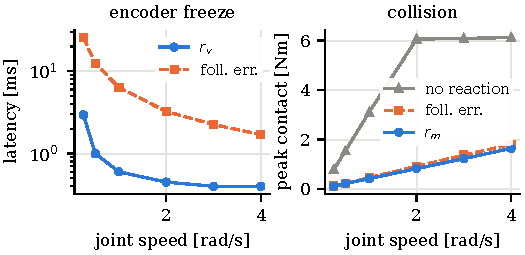
\includegraphics[width=\linewidth]{figures/sim_speed_sweep.pdf}
\caption{Speed sweep. Left: encoder-freeze detection latency (log scale).
Right: peak contact torque in a collision.}
\label{fig:sim_sweep}
\end{figure}

\subsection{Monte Carlo isolation and false alarms}
For each fault class we ran 50 trials with random model error, cruise speed
$|\dot q|\in[0.5,4]\,\si{\radian\per\second}$, and fault time; encoder
offsets were drawn from \SIrange{20}{90}{\degree} electrical and load steps
from \SIrange{0.2}{0.8}{\newton\metre}. Separately, 180 held-out normal runs of
\SI{20}{\second} each (one hour in total) measured false alarms.
\Cref{tab:sim} summarizes the results.

\begin{table}[t]
\centering
\caption{Monte Carlo simulation results (50 trials per class). Latencies in
ms, median (95th percentile). Alarm: first residual alarm. Class: time of the
final class decision.}
\label{tab:sim}
\footnotesize
\setlength{\tabcolsep}{2pt}
\begin{tabular}{@{}lcccc@{}}
\toprule
Fault & Alarm & Class & Correct & Foll.\ error \\
\midrule
Encoder freeze  & 0.27 (0.43) & 3.5 (4.3)   & 49/50 & 3.1 (9.5) \\
Encoder offset  & 0.22 (0.25) & 3.2 (3.2)   & 50/50 & 0.22$^a$ (41/50) \\
Encoder unplug  & 0.23 (0.25) & 3.2 (3.2)   & 50/50 & 0.23$^a$ \\
Phase open      & 1.3 (6.9)   & 4.2 (9.8)   & 50/50 & 67$^b$ (41/50) \\
Collision       & 2.3 (4.7)   & 42 (45)     & 50/50 & 7.0 (10.9) \\
Load step       & 1.8 (3.7)   & 42 (44)     & 50/50 & 8.1 (14.4) \\
\midrule
\multicolumn{5}{@{}l}{False alarms, 1 h normal motion: $r_v$ 0, $r_m$ 0,
foll.\ error 40/180 runs} \\
\bottomrule
\end{tabular}\\[2pt]
\footnotesize $^a$the measured position jumps, so the following error reacts
at once but cannot tell a sensor jump from a real one. $^b$the position loop
masks the lost torque for a long time.
\end{table}

Encoder faults were always detected within \SI{0.51}{\milli\second}, and
collisions within \SI{5.9}{\milli\second}. The only misclassification was an
encoder freeze at \SI{0.51}{\radian\per\second}: $r_m$ alarmed first, the
collision reflex removed the torque, the joint coasted to a stop below the
speed at which $r_v$ can see the fault, and the event was labelled
\textsc{Coll}. The reaction was still safe (zero torque), but the label was
wrong; a check of $r_v$ when control resumes, or the pulse test, would catch
it. Neither residual raised a false alarm in the held-out hour, while the
following-error check, calibrated the same way, alarmed in
\SI{22}{\percent} of the normal runs; its latency figures are therefore
optimistic.

\textbf{ROC.} Sweeping a common multiplier on each threshold, with positives
counted as detection within \SI{20}{\milli\second} and negatives as 1-second
windows of normal motion, gives an area under the curve of 0.9999 for $r_v$
on encoder faults (0.998 for the following error) and 0.9999 for $r_m$ on
collisions (0.9996). At the calibrated operating point $r_v$ and $r_m$ reach
\SI{100}{\percent} true positives with no false positives, whereas the
following-error check reaches \SI{94}{\percent} on encoder faults at a
\SI{1.2}{\percent} false-positive rate.

\textbf{Robustness.} Scaling all model-error bounds by 1.5 caused no false
alarms in 30 runs; scaling by 2 caused $r_m$ false alarms in 3 of 30 runs, and
by 3 caused $r_v$ false alarms in 3 and $r_m$ in 5 of 30 runs. The thresholds
therefore hold up to about 1.5 times the assumed parameter uncertainty, which
sets how carefully $\lambda_m$, $R$, $J$, and friction must be identified on
hardware.

% =====================================================================
\section{Experimental Validation}
\label{sec:hw}
\NOTE{Everything in this section is a placeholder until the first hardware
campaign. No numbers here are measured yet.}

\subsection{Testbed}
\TBD{Describe the actuator (motor, gearbox, driver board, MCU, encoder type
and interface), the load/obstacle fixture, the torque sensor used as ground
truth for contact torque, and logging (1~kHz logs plus high-rate capture
around events).} \TBD{Photo of the testbed.}

\subsection{Fault injection protocol}
\begin{itemize}
  \item \textsc{Enc}: (a) physical encoder unplug, (b) magnet shift by
  \TBD{deg}, (c) firmware-injected freeze and offset at random times.
  \item \textsc{Phase}: open circuit of one phase through a relay.
  \item \textsc{Coll}: impacts against a \TBD{stiff / padded} obstacle at
  \TBD{3--5} speeds, \TBD{N} trials each.
  \item \textsc{Load}: payload steps of \TBD{values}.
  \item \emph{Normal operation}, for false alarms: sine, chirp, and random
  point-to-point moves, \TBD{total hours}.
\end{itemize}
Each trial records the injection time (from a firmware flag or a sync line),
the alarm time, and the assigned class.

\subsection{Metrics}
Detection latency $t_\mathrm{alarm} - t_\mathrm{fault}$; isolation accuracy
(confusion matrix over the four classes); false-alarm rate per hour of normal
operation; peak contact torque for collisions; and ROC curves of true-positive
rate versus false-positive rate as the thresholds are swept, computed exactly
as in \cref{sec:sim}.

\subsection{Results}
\TBD{Fill in after the first hardware campaign.}

\begin{table}[t]
\centering
\caption{Hardware detection results \TBD{not yet measured}}
\label{tab:hw}
\setlength{\tabcolsep}{3pt}
\begin{tabular}{@{}lcccc@{}}
\toprule
Fault & Trials & Latency (median / max) & Correct class & Missed \\
\midrule
Encoder unplug  & \TBD{} & \TBD{} & \TBD{} & \TBD{} \\
Magnet shift    & \TBD{} & \TBD{} & \TBD{} & \TBD{} \\
Injected freeze & \TBD{} & \TBD{} & \TBD{} & \TBD{} \\
Phase open      & \TBD{} & \TBD{} & \TBD{} & \TBD{} \\
Collision (slow)& \TBD{} & \TBD{} & \TBD{} & \TBD{} \\
Collision (fast)& \TBD{} & \TBD{} & \TBD{} & \TBD{} \\
Payload step    & \TBD{} & \TBD{} & \TBD{} & \TBD{} \\
\midrule
\multicolumn{5}{@{}l}{False alarms: \TBD{} over \TBD{} h of normal motion} \\
\bottomrule
\end{tabular}
\end{table}

\begin{figure}[t]
\centering
\FIGPH{36mm}{Hardware ROC: TPR vs.\ FPR for $r_v$ (encoder faults)\\
and $r_m$ (collisions); operating point marked\\(same script as the
simulated ROC: sim/figures/sim\_roc.pdf)}
\caption{ROC curves on hardware data. \TBD{AUC values.}}
\label{fig:roc}
\end{figure}

% =====================================================================
\section{Discussion and Limitations}
\label{sec:discussion}
\begin{itemize}
  \item \emph{Low speed.} The encoder-fault signature scales with speed, so a
  frozen encoder is invisible to $r_v$ below about
  \SI{0.5}{\radian\per\second} at the joint for these parameters. High-frequency
  injection could cover standstill at the cost of noise and losses.
  \item \emph{Model error.} Dead-time distortion, $\lambda_m$ error, and
  thermal drift of $R$ set $\tau_v$; the thresholds tolerated about 1.5 times
  the assumed error bounds. Online $R$ estimation would lower $c_2$.
  \item \emph{Collision reaction.} The impact peak is set by the reflected
  inertia, so detection speed mainly prevents clamping rather than the first
  impact peak. The reflex also releases a payload for
  $T_\mathrm{coll}$ before it is recognized as \textsc{Load}; for a leg in
  stance this would need a gentler first reaction (e.g.\ admittance) instead of
  zero torque.
  \item \emph{Friction.} Friction model error appears directly in $r_m$ and
  sets the smallest detectable contact torque; a learned friction and cogging
  model would tighten this threshold.
  \item \emph{Reaction to encoder faults.} This paper stops at isolation and
  a safe state (ASC). Keeping the joint alive through sensorless control after
  an \textsc{Enc} alarm is ongoing work.
  \item \emph{Simulation fidelity.} The plant ignores cogging, magnetic
  saturation, gearbox backlash, and compliance, which hardware will add.
\end{itemize}

% =====================================================================
\section{Conclusion}
\label{sec:conclusion}
Two residuals already computable inside a PMSM joint actuator's FOC loop, a
back-EMF voltage residual and a generalized-momentum observer, have
complementary sensitivity that isolates encoder faults from mechanical events
without extra sensors. In simulation with up to \SI{30}{\percent} model error,
the scheme isolated 299 of 300 injected faults, raised no false alarms in an
hour of normal motion, detected encoder faults within \SI{0.51}{\milli\second},
and detected collisions about three times faster than a following-error check.
\TBD{Hardware summary sentence.} Future work extends the scheme to
encoder-fault-tolerant control so that a humanoid joint can keep operating
after a sensor fault.

\bibliographystyle{IEEEtran}
\bibliography{refs}

\end{document}
